%% LaTeX template for the science justification & technical
%% feasibility to be submitted as part of a TESS Guest Investigator
%% Program proposal. This template is based on the proposal template
%% used by the NuSTAR mission.
%%
%% TESS Guest Investigator Proposal Cycle 2 template
%% V1.0
%% 2017-08-04
%% V1.1
%% 2019-02-07

%%%%%%%%%%%%%%%%%%%%%%%%%%%
%%%%% DOCUMENT FORMAT %%%%%
%%%%%%%%%%%%%%%%%%%%%%%%%%%

%% The default font was chosen to be easily readable while allowing
%% sufficient material to be included.

%% Please note that the proposal will be printed on US Letter size paper,
%% 8.5 in x 11 in, and that formatting the text for other sizes will
%% generally cause layout problems and may result in text being cut
%% off near the edges. PLEASE DO NOT CHANGE THE 'LETTERPAPER' OPTION
%% IN THE DOCUMENTCLASS COMMAND.

%%%%%%%%%%%%%%%%%%%%%%%%%%%%%%%%%%%%%%%%%%%%%%
%%%%% Default format: 11pt single column %%%%%
%%%%%%%%%%%%%%%%%%%%%%%%%%%%%%%%%%%%%%%%%%%%%%

%% NOTE: NASA ROSES requires body font size to be no smaller than 15
%% characters per inch (equivalent to Times Roman 12 point).
%%
%% Minimum margin size is 1 inch from top, bottom, and sides.

\documentclass[letterpaper,11pt]{article}

%%%%%%%%%%%%%%%%%%%%%%%%%%%%%%%%%%
%%%%% HOW TO INCLUDE FIGURES %%%%%
%%%%%%%%%%%%%%%%%%%%%%%%%%%%%%%%%%

%% Please see the ``Included packages'' section below.

%%%%%%%%%%%%%%%%%%%%%%%%%%%%%
%%%%% Included packages %%%%%
%%%%%%%%%%%%%%%%%%%%%%%%%%%%%

\usepackage{graphics,graphicx}
\usepackage{aas_macros}
%\usepackage[comma,authoryear]{natbib}
%\bibpunct{(}{)}{;}{a}{}{;}

\usepackage{caption}
\usepackage{subcaption}
\usepackage{cancel}

\usepackage{fontspec}
\usepackage[T1]{fontenc}
\usepackage{newtxsf}
\setmainfont{Fira Sans Book}[Scale=0.95]


\usepackage[backref,breaklinks,colorlinks,urlcolor=blue,citecolor=blue,linkcolor=blue]{hyperref}
\bibliographystyle{plain}
%\bibliographystyle{yahapj}
\usepackage{cleveref}
\usepackage{enumerate}
\usepackage{amsmath,amssymb}
\usepackage{bm}
\usepackage{color}
\usepackage[utf8]{inputenc}

\newcommand{\prob}{{\rm prob}}
\newcommand{\qN}{\{q_i\}_{i=1}^N}
\newcommand{\qM}{\{q_{im}\}_{i=1,m=0}^{N,M}}
\newcommand{\yN}{\{y_i\}_{i=1}^N}

\newcommand{\kms}{ \textrm{km s}^{-1} }

\newcommand{\vM}{\mathsf{M}}
\newcommand{\vD}{\mathsf{D}}
\newcommand{\vR}{\mathsf{R}}
\newcommand{\vC}{\mathsf{C}}
\newcommand{\fM}{ \vec{{\bm M}}}
\newcommand{\fMi}{M_i}
\newcommand{\fD}{ \vec{{\bm D}}}
\newcommand{\fDi}{D_i}
\newcommand{\fR}{ {\bm R}}
\newcommand{\dd}{\,{\rm d}}
\newcommand{\trans}{\mathsf{T}}
\newcommand{\teff}{T_\textrm{eff}}
\newcommand{\logg}{\log g}
\newcommand{\Z}{[{\rm Fe}/{\rm H}]}
\newcommand{\A}{[\alpha/{\rm Fe}]}
\newcommand{\vsini}{v \sin i}
\newcommand{\matern}{Mat\'{e}rn}
\newcommand{\HK}{$\textrm{H}_2$O-K2}
\newcommand{\cc}[2]{c_{#2}^{(#1)}} 

\newcommand{\flam}{f_\lambda}
\newcommand{\vt}{ {\bm \theta}}
\newcommand{\vT}{ {\bm \Theta}}
\newcommand{\vp}{ {\bm \phi}}
\newcommand{\vP}{ {\bm \Phi}}
\newcommand{\cheb}{ \vp_{\mathsf{P}}}
\newcommand{\chebi}[1]{ \vp_{\textrm{Cheb}_{#1}}}
\newcommand{\Cheb}{ \vP_{\textrm{Cheb}}}
\newcommand{\Chebi}[1]{ \vP_{\textrm{Cheb}_{\ne #1}}} 
\newcommand{\cov}{ \vp_{\mathsf{C}}}
\newcommand{\covi}[1]{ \vp_{\textrm{cov}_{#1}}} 
\newcommand{\Cov}{ \vP_{\textrm{cov}}}
\newcommand{\Covi}[1]{ \vP_{\textrm{cov}_{\ne #1}}} 

\newcommand{\allParameters}{\vT} 
\newcommand{\nuisanceParameters}{\vP} 

\newcommand{\KK}{\mathcal{K}}
\newcommand{\Kglobal}{\KK^{\textrm{G}}}
\newcommand{\Klocal}{\KK^{\textrm{L}}}

\newcommand{\Gl}{Gl\,51}
\newcommand{\PHOENIX}{{\sc Phoenix}}

% Appendix commands
\newcommand{\wg}{\mathbf{w}^\textrm{grid}}
\newcommand{\wgh}{\hat{\mathbf{w}}^\textrm{grid}}

\newcommand{\Sg}{\mathbf{\Sigma}^\textrm{grid}}


\newcommand{\todo}[1]{ \textcolor{blue}{\\TODO: #1}}
\newcommand{\comm}[1]{ \textcolor{red}{SA: #1}}
\newcommand{\hili}[1]{ \textcolor{green}{#1}}
\newcommand{\ctext}[1]{ \textcolor{blue}{\% #1}}

%% Feel free to modify the included packages list to use your
%% favorite packages.

%% In the graphics and graphicx packages, Postscript and eps figures
%% can be included using the \includegraphics command. The graphics
%% package is part of standard LaTeX2e and provides a basic way of including a
%% figure. The graphicx package is not standard, but extends the
%% \includegraphics command to make it more user-friendly. If graphicx
%% is not available on your system please remove it from the list of
%% included packages above.

%% Syntax:
%% In the graphics package:
%%
%% \begin{figure}
%% \includegraphics[llx,lly][urx,ury]{file}
%% \end{figure}
%%
%% where ll denotes 'lower left' and ur 'upper right' and the x and y
%% values are the coordinates of the PostScript bounding box in
%% points. There are 72 points in an inch.
%%
%% In the graphicx package:
%%
%% \begin{figure}
%% \includegraphics[key=val,key=val,...]{file}
%% \end{figure}
%%
%% where some of the useful keys are: angle, width, height,
%% keepaspectratio (='true' or 'false') and scale. Bounding box values
%% can be given as [bb=llx lly urx ury].
%%
%% In either case you have to use LaTeX figure placement commands to
%% position the figure on the page; \includegraphics will not do
%% that. Both these commands also have other options that are listed
%% in the LaTeX manual (for the graphics package) and in 'The LaTeX
%% Graphics Companion' (for the graphicx package).



%%%%%%%%%%%%%%%%%%%%%%%%%%%
%%%%% Page dimensions %%%%%
%%%%%%%%%%%%%%%%%%%%%%%%%%%

\setlength{\textwidth}{6.5in}
\setlength{\textheight}{9in}
\setlength{\topmargin}{-0.0625in}
\setlength{\oddsidemargin}{0in}
\setlength{\evensidemargin}{0in}
\setlength{\headheight}{0in}
\setlength{\headsep}{0in}
\setlength{\hoffset}{0in}
\setlength{\voffset}{0in}



%%%%%%%%%%%%%%%%%%%%%%%%%%%%%%%%%%
%%%%% Section heading format %%%%%
%%%%%%%%%%%%%%%%%%%%%%%%%%%%%%%%%%

\makeatletter
\renewcommand{\section}{\@startsection%
{section}{1}{0mm}{-\baselineskip}%
{0.5\baselineskip}{\normalfont\Large\bfseries}}%
\makeatother

%%%%%%%%%%%%%%%%%%%%%%%%%%%%%%%%%%%%%
%%%%% Some Useful Abbreviations %%%%%
%%%%%%%%%%%%%%%%%%%%%%%%%%%%%%%%%%%%%
\newcommand{\tess}{{\it TESS}}
\newcommand{\jwst}{{\it JWST}}
\newcommand{\kepler}{{\it Kepler}}
\newcommand{\ktwo}{{K2}}
\newcommand{\hst}{{\it HST}}
\newcommand{\msun}{$M_{\odot}$}
\newcommand{\rsun}{$R_{\odot}$}
\newcommand{\lsun}{$L_{\odot}$}
\newcommand{\re}{$R_{\oplus}$}
\newcommand{\me}{$M_{\oplus}$}
\newcommand{\rj}{$R_{\textrm{\scriptsize Jup}}$}
\newcommand{\mj}{$M_{\textrm{\scriptsize Jup}}$}
\newcommand{\ms}{m~s$^{-1}$}


%\include{JournalAbbr}

%%%%%%%%%%%%%%%%%%%%%%%%%%%%%
%%%%% Start of document %%%%%
%%%%%%%%%%%%%%%%%%%%%%%%%%%%%

\begin{document}
\pagestyle{plain}
\pagenumbering{arabic}


%%%%%%%%%%%%%%%%%%%%%%%%%%%%%
%%%%% Title of proposal %%%%%
%%%%%%%%%%%%%%%%%%%%%%%%%%%%%

\begin{center}
\bfseries\uppercase{%
%%
%% ENTER TITLE OF PROPOSAL BELOW THIS LINE
Mitigating exoplanet radius biases from wavelength dependence of starspot contrast
%%
%%
}
\end{center}



%%%%%%%%%%%%%%%%%%%%%%%%%%%%%%%%%%%%%%%%%
%%%%% Body of science justification %%%%%
%%%%% and technical feasibility     %%%%%
%%%%%%%%%%%%%%%%%%%%%%%%%%%%%%%%%%%%%%%%%

\section{Introduction}

Recent work has shown that ignoring starspots systematically biases measurements of exoplanet radii \cite{2018ApJ...853..122R}.  Here we propose a strategy for mitigating starspot-induced exoplanet radius biases, based on a large sample of spotted stars observed in \tess\ Cycle 2.  The approach will deliver constraints on both the typical starspot coverage fraction and the typical starspot temperature contrast, as a function of spectral type and rotation rate.  This mapping can then serve as a ``lookup table'' for practitioners to gauge the extent to which a given source is likely to suffer from starspot-induced exoplanet radius biases.  No such reliable lookup table presently exists for main sequence stars, owing to the inability of differential lightcurves to account for \emph{total} starspot coverage fractions \cite{2018ApJ...865..142B}.  This program will leverage the \tess\ Cycle 2 overlap with the \kepler\ prime field and portions of \ktwo\ fields.

\section{Scientific Justification: The Transit Light Source Effect}
The diminution of flux arising from occultations of the stellar disk contains information the relative sizes of the occulting bodies.  A commonsense exoplanet heuristic dictates that the relative transit depth $D$ equals the ratio of the bodies' projected areas ($R_p^2/R_\star^2$).  Additional correction factors account for limb darkening \cite{2002ApJ...580L.171M}.  Starspots on a stellar surface can exhibit spatial segregations
that yield \emph{unocculted starspots}: spots that are present on the surface but are not traversed during transits.  These unocculted starspots confound the mapping of transit depth to planet radius: a planet ``looks bigger'' than it really is if it blocks the brighter-on-average flux of the stellar disk \cite{2018AJ....156...91M}.  \textbf{You cannot measure a planet radius without making some assumptions about the extent, contrast, and distribution of starspots.}

The prevailing assumption within the exoplanet community has been that starspot covering fractions are small enough---as in Sunspots---to be ignored.  New theoretical models \cite{2018ApJ...853..122R} and observational evidence \cite{2016MNRAS.463.2494F} indicate that starspot covering fractions are large enough to bias transit depths beyond the level of precision of \kepler\ and \tess.  This so-called ``Transit Light Source Effect'' (TLSE) can bias derived exoplanet radii up to 17\% in the \tess\ bandpass, and can bias derived exoplanet \emph{densities} up to 50\%, since the radius error propagates into volume error with a factor of 3.  Therefore, TLSE threatens placement and interpretation of the exoplanet mass-radius relation science requirements of the \tess\ mission.  The interpretation of \jwst\ exoplanet transmission spectroscopy is also at risk \cite{2019AJ....157...11W}.

\section{Analysis Plan}

\textbf{Kepler and TESS perceive different starspot contrasts.}

Starspots emit light, which is often parameterized as \emph{spot contrast}, $c$, where 0 means the spots are non-emitting, and $c=1$ means the spot matches the specific intensity of the ambient photosphere.  Spot contrast is wavelength dependent ($c_\lambda$) and can be thought of as possessing a characteristic spot temperature, $T_{spot}<T_{phot}$ that parameterizes the wavelength dependence of the contrasts.  The analysis technique proposed here leverages the different wavelength dependence of the \kepler\ and \tess\ system throughputs to directly measure the ratio of the spot contrasts in their respective bandpasses.  The spot contrast ratio---evaluated at these two pairs of bandpasses---provides a unique solution\footnote{Operationally, integrating the specific intensity $I_\lambda(T_{spot})$ over the system throughputs produces the expected contrast ratios.  For now we assume $I_\lambda(T_{spot})$ can be approximated as a cooler stellar photosphere, such as the \texttt{PHOENIX} model grid \cite{2013A&A...553A...6H}, an inexact but adequate assumption for the large bandpasses.} to $T_{spot}(\mathrm{SpT},\;P_{\mathrm{rot}})$.

\textbf{Spot-induced modulation amplitudes depend on contrast.}
Rotationally-modulated lightcurves exhibit semi-sinusoidal undulations as starspots (or spot groups) enter and exit the projected stellar disk.  The most-spotted projected hemisphere is directed towards the observer at the moment of the lightcurve minimum, and the least-spotted projected hemisphere at lightcurve maximum.  The amplitude of the lightcurve, therefore, equals the difference in starspot coverage fractions $\Delta f_{spot} \equiv f_{max}-f_{min}$ between the most-and-least spotted projected hemispheres weighted by the spot contrast: $ A_\lambda = \Delta f_{spot} \cdot (1-c_\lambda)$.  Therefore the ratio of \tess\ to \kepler\ amplitudes yields a constraint independent of the actual spot coverage fraction:

$$ \frac{A_{TESS}}{A_{Kepler}} = \cancel{\frac{\Delta f_{spot}}{\Delta f_{spot}}} \cdot \frac{1-c_{TESS}}{1-c_{Kepler}} $$

Recent stellar surface inhomogeneity modeling \cite{2018ApJ...853..122R, 2018ApJ...868..143G, 2018ApJ...865..142B} has yielded coarse scaling factors $\zeta$ for estimating the total starspot surface coverage fraction from the observed lightcurve amplitude $f_{spot}$, yielding $ p(f_{spot}) = \zeta \cdot A $, where $\zeta$ represents a probability distribution with values typically between 1 and 50, depending on the degree of assumed starspot longitudinal symmetry.  Equipped solely with \tess-measured lightcurve amplitudes, we can provide what practitioners seek: a per-star estimate of $f_{spot}$ and $T_{spot}$.

\textbf{Distinguishing Kepler/K2 and TESS amplitudes with statistically similar samples}

Ideally, we would have simultaneously observed the same targets with \kepler\ and \tess\ to measure the contrast for individual stars.  Since this observational strategy was not possible for a large number of stars, we instead construct statistical subsamples of stars that are identical in every way, except for their observation band.

The main two factors that affect spot-modulation lightcurve amplitudes are effective temperature (\emph{i.e.} mass), and rotation period (\emph{i.e.} stellar activity/magnetic fields) \cite{2014ApJS..211...24M}.  Other important-albeit-unknown factors like stellar inclination angle and multiplicity are statistically identical between the \tess\ and \kepler\ samples.  We, therefore, propose to follow \cite{2014ApJS..211...24M} by constructing plots of amplitude versus period, subdivided into bins of effective temperature.  The two samples should look identical in these plots, but the locus of \tess\ sources is expected to fall below the \kepler\ sample, as in panel D of Figure \ref{fig:predictAmps}.

\begin{figure}[hbt!]
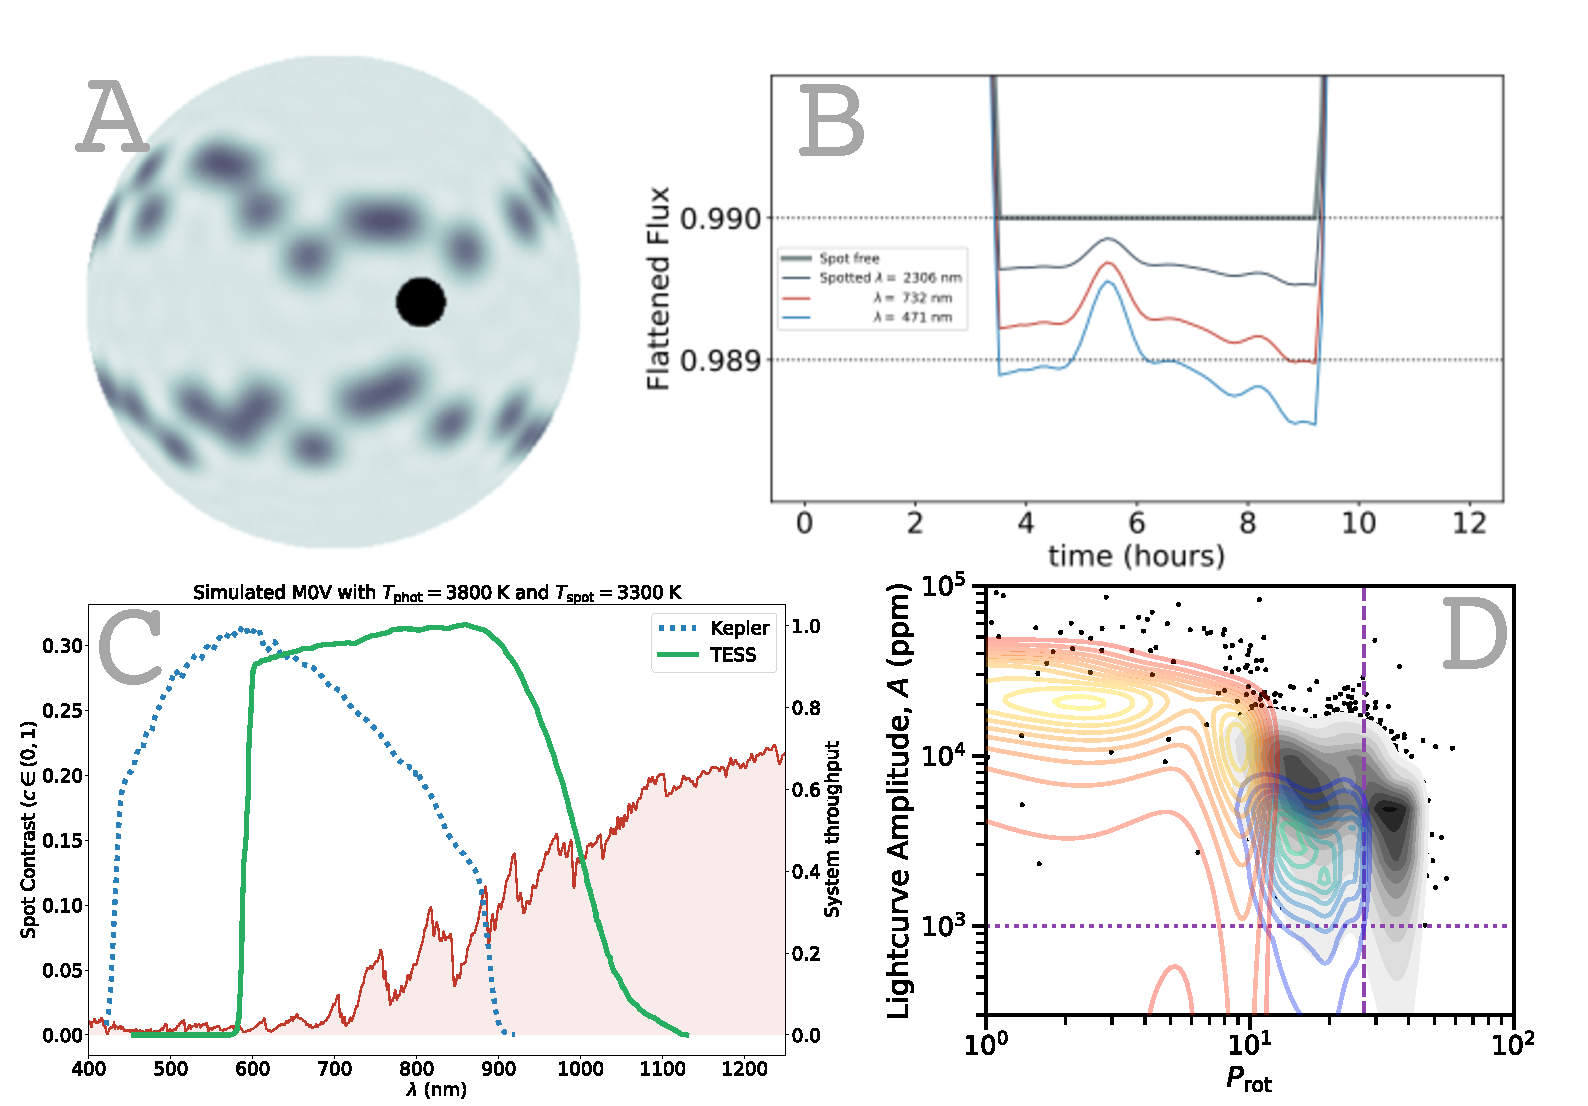
\includegraphics[width=0.95\textwidth]{figures/multi_panel.pdf}
\caption{\texttt{A)} Schematic of a planet ($R_p = 0.1 R_\star$) transiting a star with unocculted starspots as the star moves from left to right.  \texttt{B)} The resulting transit depth shows a systematic bias and a wavelength dependence due to starspots. \texttt{C)} Illustration of TLSE, \texttt{D)} Prediction for \tess\ amplitudes (colorful contours) relative to the \kepler\ sample (gray shaded background contours and black points) for $4000 < T_{phot} (K) < 4500$ \cite{2014ApJS..211...24M}.}
\label{fig:predictAmps}
\end{figure}

\tess\ Cycle 2 will have significant overlap with both the \kepler\ prime field (up to 3 sectors of overlap) and 16438 source in the northern edges of \ktwo\ campaign fields (K. Col\'on, priv. comm.).  This overlap sample offers an independent check on any statistical biases since the exact same stars can be compared.  The fact that observations are not contemporaneous adds some \emph{cosmic variance}, but on average stars will enter and exit stellar activity cycles in equal measure, injecting per-star variance, but keeping the subsample mean amplitudes the same.

\section{Technical Feasibility}

Measuring periods and amplitudes of \kepler\ and \tess\ lightcurves is a routine operation, with relatively low risk.  The PI has significant experience determining amplitudes with a Fourier-based decomposition technique in young stars observed in \ktwo.  The derived periods and amplitudes need not be \emph{perfect}, so long as the biases are about the same in both the \kepler\ and \tess\ subsamples.

The yield of spotted stars in \tess\ will number in the hundreds of thousands.  The \tess\ mission was designed to target cool main sequence stars with an abundance of K and M dwarfs.  This program will focus on the rapidly rotating stars ($P_{rot}<20$ days), which exhibit relatively large amplitudes ($A>2000$ ppm), illustrated in panel D of Figure \ref{fig:predictAmps}.  This program will attempt---on a best effort basis---to measure the slowest rotating stars, which have periods much longer than the typical observation window of 27$-$54 days, and amplitudes comparable to the precision limits of \tess; these slow rotating sources must reside near the continuous viewing zone in the North Ecliptic Pole to have any hope of detecting spot modulation.

One potential risk to this program is the that the \kepler\ and \tess\ populations will be statistically different from each other in their unobserved properties, confounding the assumption that the samples' only difference is the observation bandpass.  For example, metallicity, age, extinction, and stellar background contamination may all be different between the \kepler\ samples and \tess\ samples.  This risk is alleviated by the subsample of \kepler\ sources reobserved in \tess\ Cycle 2.

\section{Expected Impact}

The main deliverable of this work will be a probabilistic assessment of the starspot temperature and starspot coverage faction for every star with a measured starspot modulation period and amplitude in \tess.  These probability distributions will empower exoplanet researchers to correct for biases in exoplanet transit radii.  The probability distributions will reflect all the available information garnered from \tess, and reasonable assumptions about starspot geometrical distributions.

Stellar surface structures serve as a stepping stone for brown dwarf cloud modeling, a poorly understood phenomenon that will inform our understanding of exoplanet spectroscopy.  The proposed work will demonstrate how to gain insights about probable surface structures in the presence of significant geometrical degeneracies.

The starspot properties are also of intrinsic astrophysical interest.  Trends in $T_{spot}$ with rotation rate and mass can reveal important clues to stellar activity, magnetic fields, and stellar atmospheres.  This work will directly address starspot-induced scatter and bias in isochronal-derived stellar ages \cite{2015ApJ...807..174S, 2017ApJ...836..200G}.

\section{Work Plan}

PI Gully-Santiago will carry out the data analysis using custom scripts that build upon the heritage of the \kepler\ data analysis ecosystem, including \texttt{lightkurve}, \texttt{astropy}, \texttt{celerite}, \texttt{BombScargle}, \texttt{PyTorch}, and \texttt{bokeh}.  The PI will first apply these scripts to Kepler/K2 lightcurves while in the role as a support scientist at the Kepler/K2 Guest Observer Office.  The PI will relocate to the University of Texas at Austin in February 2020 as a Research Fellow.  UT Austin undergraduate and graduate students will lead the application of TESS-adapted scripts to \tess\ FFI lightcurves with \texttt{TESS-cut} and \texttt{elenor}.  Half of the funding will go to 1 undergraduate and 1 graduate student Summer 2020 salary, and 0.3 FTE to support the PI.  All reproducible scripts---including Jupyter Notebook tutorials---will be publicly available and developed openly on GitHub.  MGS will provide students with an interactive \texttt{bokeh} tool to visualize periodic lightcurve structures.  This tool will leverage the PI's familiarity with \texttt{bokeh} to aid rapid visual spot-checking of the multidimensional analysis output.  Finally, a High-Level Science Product (HLSP) will be delivered to MAST that contains the following information for each star found to possess detectable starspot-induced lightcurve modulation: 1) the period or periods, 2) an iteratively determined outlier mask of stellar flares, occultations, or spurious data artifacts, 3) a background-star amplitude-dilution estimate, 4) a probability distribution for the spot temperature and coverage fraction, 5) addition model fitting metadata.  MGS will co-advise---with Co-I C. Morley---students in the writeup of the paper(s), authored and/or coauthored by students.


\newpage

\bibliography{tessgi_gully_cycle2}


\end{document}
